% !TeX program = pdflatex
\documentclass[tikz,border=8pt]{standalone}
\usepackage{tikz}\usetikzlibrary{arrows.meta}
\definecolor{FigureBlue}{HTML}{2563EB}\definecolor{FigureOrange}{HTML}{EA580C}
\begin{document}
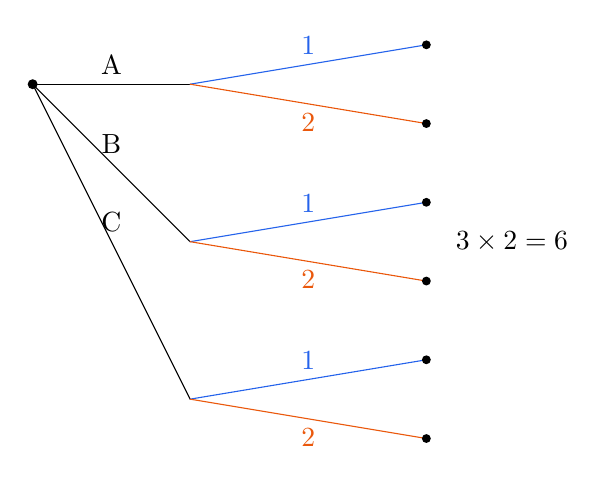
\begin{tikzpicture}[>=Stealth,line cap=round]
  \coordinate (R) at (0,0); \foreach \i/\lab in {1/A,2/B,3/C}{\coordinate (N\i) at (2,2-2*\i);\draw (R)--(N\i) node[midway,above] {\lab};}
  \foreach \i in {1,2,3}{\coordinate (L\i-A) at (5,2.5-2*\i);\coordinate (L\i-B) at (5,1.5-2*\i);\draw[FigureBlue] (N\i)--(L\i-A) node[midway,above] {$1$};\draw[FigureOrange] (N\i)--(L\i-B) node[midway,below] {$2$};\fill (L\i-A) circle (1.6pt);\fill (L\i-B) circle (1.6pt);}
  \fill (R) circle (1.8pt); \node[right] at (5.25,-2) {$3\times2=6$};
\end{tikzpicture}
\end{document}
